\documentclass[12pt,a4paper]{article}
%% ntts2019abstract..tex - https://ec.europa.eu/eurostat/cros/system/files/ntts2019abstract_tex.zip
%% TEMPLATE FOR NTTS 2019 CONFERENCE
%% This LaTex source file is (coarsely) following the corresponding DOT template document of
%% the conference (https://ec.europa.eu/eurostat/cros/system/files/ntts2019abstract.dot)
%% Prepared by J.Grazzini (Eurostat, unit B1)

\def\thisfile{ntts2019abstract}

%% WHO ARE YOU: LIST THE AUTHORS HERE
\def\theauthors{
\color{red}{\parbox{0.9\textwidth}{ % delete this line when submitting
\centering{\textbf{To allow for blinded review:}}
~\\
\centering{\textbf{do NOT indicate author information or affiliation}}
}}% delete this line when submitting
}

%% WHAT IS YOUR PAPER ABOUT: PUT YOUR TITLE HERE
\def\thetitle{
\colorbox{yellow}{\parbox{\textwidth}{ % delete this line when submitting
\textbf{Title – exactly as indicated in the “title” field}
}}% delete this line when submitting
}

%% TELL US MORE... THROUGH KEYWORDS!
\def\thekeywords{
\colorbox{yellow}{ % delete this line when submitting
\textit{Exactly as indicated in the “keyword” fields, separated by commas.}
}% delete this line when submitting
}

%% PLEASE KEEP AT LIST THESE SETTINGS
\def\thepaperheight{29.9cm} 	% original: {11.99in}
\def\thepaperwidth{21.08cm} 	% 		{8.3in}
\def\theleft{2.79cm} 			% 		{1.1in}
\def\theright{2.99cm} 			%		{1.18in}
\def\thetop{1.7cm} 			% 		{0.51in}
\def\thebottom{1.6cm} 		% 		{0.71in}
\def\theheadheight{2.54cm} 	% 		(1in}

\usepackage[
   a4paper,
   paperheight=\thepaperheight,
   paperwidth=\thepaperwidth,
   left=\theleft,
   right=\theright,
   top=\thetop,
   bottom=\thebottom,
   headheight=\theheadheight
]{geometry} % in particular, do not change the dimensions of the document

\usepackage{fancyhdr}

%\cfoot{ {\fontsize{8pt}{9.6pt}\selectfont 6\par}}

%% NO HEADING...
%%\fancyhead[RE]{\headreport}
%%\fancyhead[RO,LE]{\bfseries\thepage}
%%\fancyhead[LO]{\nouppercase{\rightmark}} %{\markright} %{\sectionmark}

\pagestyle{fancy}
\fancyhf{}

% you can use hyperref as set below once the colorboxes are gone...
% \usepackage[pdfauthor={\theauthors}, pdftitle={\thetitle}]{hyperref}
% otherwise simply stick to that one
\usepackage{hyperref}

\hypersetup{colorlinks=true,       % false: boxed links; true: colored links
    % linkcolor=blue,          % color of internal links
    citecolor=red,        % color of links to bibliography
    filecolor=magenta,      % color of file links
    urlcolor=cyan           % color of external links
}
%% or:
% \usepackage[hidelinks]{hyperref} % make links black

\usepackage{sectsty}
\usepackage{setspace}

\renewcommand{\headrulewidth}{0pt}
\setlength{\topsep}{0pt}\setlength{\parindent}{0pt}

\renewcommand{\arraystretch}{1.3}

%% depths for Sections 
% 1) Section
% 1.1) SubSection
% 1.1.1) SubSubSection
% 1.1.1.1) Paragraph
\setcounter{tocdepth}{4}
\setcounter{secnumdepth}{4}

% depths for nested lists created by \begin{enumerate}
\usepackage{enumitem}
\setlistdepth{9}
\renewlist{enumerate}{enumerate}{9}
	\setlist[enumerate,1]{label=\arabic*)}
	\setlist[enumerate,2]{label=\alph*)}
	\setlist[enumerate,3]{label=(\roman*)}
	\setlist[enumerate,4]{label=(\arabic*)}
	\setlist[enumerate,5]{label=(\Alph*)}
	\setlist[enumerate,6]{label=(\Roman*)}
	\setlist[enumerate,7]{label=\arabic*}
	\setlist[enumerate,8]{label=\alph*}
	\setlist[enumerate,9]{label=\roman*}
\renewlist{itemize}{itemize}{9}
	\setlist[itemize]{label=$\cdot$}
	\setlist[itemize,1]{label=\textbullet}
	\setlist[itemize,2]{label=$\circ$}
	\setlist[itemize,3]{label=$\ast$}
	\setlist[itemize,4]{label=$\dagger$}
	\setlist[itemize,5]{label=$\triangleright$}
	\setlist[itemize,6]{label=$\bigstar$}
	\setlist[itemize,7]{label=$\blacklozenge$}
	\setlist[itemize,8]{label=$\prime$}

% that's for generating directly PDF documents using pdfLaTex instead of LaTex alone
\newif\ifpdf\ifx\pdfoutput\undefined\pdffalse\else\pdfoutput=1\pdftrue\fi
\newcommand{\pdfgraphics}{\ifpdf\DeclareGraphicsExtensions{.pdf,.png,.tif,.jpg}\else\fi}

%% KEEP THIS FOR THE EXAMPLES BELOW TO RUN...OR RUN YOUR OWN
% \usepackage[boxed]{algorithm2e}
\usepackage{algorithm}
%\usepackage{algorithmic}
\usepackage[noend]{algpseudocode}
\makeatletter\def\BState{\State\hskip-\ALG@thistlm}\makeatother

%% DEAL WITH THE BIBLIOGRAPHY

% that's what we use here for the bibliography
\usepackage[numbers]{natbib}
% see https://gking.harvard.edu/files/natnotes2.pdf
\newcommand*{\doi}[1]{DOI: \href{https://doi.org/\detokenize{#1}}{\detokenize{#1}}} 
\newcommand*{\arxiv}[1]{arXiv: \href{https://arxiv.org/abs/\detokenize{#1}}{\detokenize{#1}}} 


%% If you are compiling using biblatex
%\usepackage[
%    backend=biber,
%    style=authoryear,
%    natbib=true,
%    url=true, 
%    doi=true,
%    eprint=false, 
%    sorting=ynt
%]{biblatex}
%\addbibresource{\thisfile.bib}

%% THANKS!

%% SUGGESTED PACKAGES - DO WTF YOU WANT HERE 

\usepackage[utf8]{inputenc}
\usepackage[T1]{fontenc}

\usepackage{amsmath}
\usepackage{latexsym}
\usepackage{amsfonts}
\usepackage[normalem]{ulem}
\usepackage{array}
\usepackage{amssymb}

\ifpdf
\usepackage[pdftex]{graphicx}
\else
\usepackage{graphicx}
\fi

%\graphicspath{
%
%}

\usepackage{float}
%\usepackage{subfloat}
\usepackage{subfig}
% \usepackage[list=true]{subcaption} % cannot be used conjointly with subfig
\usepackage{wrapfig}
\usepackage{wasysym}
\usepackage[svgnames,table]{xcolor}
\usepackage{longtable} % long tabulars
\usepackage{adjustbox}
\usepackage{alltt} % verbatim 
\usepackage{changepage}
\usepackage{hhline}
\usepackage{multicol}
\usepackage{tabto}
\usepackage{multirow}
%\usepackage{ragged2e}
%\usepackage{tikz}
%\usepackage{makecell}
%\usepackage[toc,page]{appendix}

\urlstyle{same}


 %% HEADER
\title{
\vspace{-5ex}
\thetitle
\vspace{-2ex}
}
\author{
\theauthors
\vspace{-5ex}
}
\date{}


%% YOUR DOCUMENT STARTS HERE

\begin{document}
\cfoot{\thepage} % keep pages numbered

%% PLEASE KEEP THIS FORMATTING
\sectionfont{\large\textsc}
%\sectionfont{\large\MakeUppercase}
%%

\maketitle

{\fontsize{10pt}{12.0pt}\selectfont \textbf{\uline{Keywords}:} \thekeywords\par}\par

{~\\
{\color{red} \noindent \uline{Instructions}:
The headings “introduction”, “methods”, “results” and “conclusions” may be replaced by other expressions, if there are compelling reasons to do so. The abstract should be reasonably self-contained; an abstract should normally have actual results/findings presented in a compact but intelligible format. Abstracts failing to contain such basic information would only be accepted under exceptional circumstances.

Please respect the overall structure. Replace all text highlighted in \colorbox{yellow}{yellow} with the appropriate information corresponding to your abstract. Depending on your need for subsections, either replace or remove all text highlighted in \colorbox{green}{green}.

Prior to submission, please delete all red instruction text, and remove all highlighting from the document. The colour of all text in the abstract should be black, non- highlighted.

Please bear in mind that this is an abstract; (i) the minimum length allowed (to allow reviewers to take an informed decision on your abstract) is 2 pages; (ii) the maximum length allowed is 4 pages. (A focus on the salient aspects of your abstract is required; details could be saved for the full paper to be submitted after the presentation at the conference).
}}

\section{ Introduction}
\addcontentsline{toc}{section}{Introduction}
\colorbox{yellow}{Text.}\par
\subsection{\colorbox{green}{Subtitle if needed (please delete otherwise)}}
\colorbox{green}{Subsection text}
\subsection{\colorbox{green}{Subtitle if needed (please delete otherwise)}}
\colorbox{green}{Subsection text}

\section{Methods}
\addcontentsline{toc}{section}{Methods}
\colorbox{yellow}{Text.}\par
\subsection{\colorbox{green}{Subtitle if needed (please delete otherwise)}}
\colorbox{green}{Subsection text}
\subsection{\colorbox{green}{Subtitle if needed (please delete otherwise)}}
\colorbox{green}{Subsection text}


\colorbox{green}{
Run your equation(s) with whatever \textit{math} package you prefer:
}
\begin{equation}\label{eq:fermat-knew-it}
\forall  n \in I\!\!N, n \geq 3, \exists x, y, z \in I\!\!N \mid x^n + y^n = z^n \quad \text{(or maybe not actually)}
\end{equation}
\colorbox{green}{and possibly refer them as Eq.~(\ref{eq:fermat-knew-it}) or Equation~(\ref{eq:fermat-knew-it}).}

\begin{small}
\begin{algorithm}[htbp]
\caption{Pseudo code for reviewing process}\label{alg:acceptance}
\begin{algorithmic}[1]
\Procedure{Acceptance}{paper, committee}
\State $\textit{reviewers} \gets \text{randomly select } \{(i,j) \mid i,j \in  \{1, \cdots, \#\{\textit{committee}\}\}, i \neq j \}$
\State $\textit{reviews} \gets 2 \times 1 \text{ array of } \textit{False}$
\BState \emph{reviewing round}:
\For {$i \in \textit{reviewers }$}
\If {$paper \text{ reads well for } \textit{committee}(i) $}
\State $\textit{review}(i) \gets \textit{True}$.
\Else \text{ do nothing}
\EndIf
\EndFor
\BState \emph{evaluation round}:
\If {$\textit{reviews}(i) \text{ is } \textit{False} \text{ for all } i \in \textit{reviewers}$}
\State \textbf{goto} \emph{hell}.
\ElsIf {$\textit{reviews}(i) \text{ is } \textit{True} \text{ for all } i \in \textit{reviewers}$}
\State \textbf{goto} \emph{Bruxelles}
\Else \textbf{ goto} \emph{revision round}
\EndIf
\BState \emph{revision round}:
\State $\textit{reviser} \gets \text{randomly select } \{i \mid i \in  \{1, \cdots, \#\{\textit{committee}\}\}, i \not\in \textit{reviewers} \}$
\If {$paper \text{ reads well for } \textit{committee(reviser)} $}
\State \textbf{ goto} \emph{Bruxelles}
\ElsIf{\textit{committee(reviser)} \text{ has no opinion and likes inifinite loop}}
\State \textbf{ goto} \emph{reviewing round}
\Else \textbf{ goto} \emph{hell}
\EndIf
\BState \emph{hell} 
\State \text{Try again at NTTS 2021!}
\BState \emph{Bruxelles (some people also call it hell)}:
\State \text{See you at NTTS 2019!}
\EndProcedure
\end{algorithmic}
\end{algorithm}
\end{small}

\colorbox{green}{
You can describe your home-made algorithm(s) like in Algorithm~\ref{alg:acceptance} (also referred as Alg.~\ref{alg:acceptance}).
}


\section{Results}
\addcontentsline{toc}{section}{Results}

\colorbox{green}{Please remember to always refer to the table(s) and figure(s) in the text; see for instance}

\colorbox{green}{reference to Table~\ref{tab:dumb} (or Tab.~\ref{tab:dumb}) and Figure~\ref{fig:dumber} (or Fig.~\ref{fig:dumber})}

\begin{table}[htbp]
\begin{center}
	\caption{\colorbox{green}{Table caption – above the table}}\label{tab:dumb}
	\begin{tabular}{|*{6}{p{0.14\textwidth}|}}
	\hline 
	& & &  & & \\
	\hline 
	& & & & & \\
	\hline 
	& & & & & \\
	\hline
	\end{tabular}
\end{center}
\end{table}

\begin{figure}[htbp]
\begin{center}
		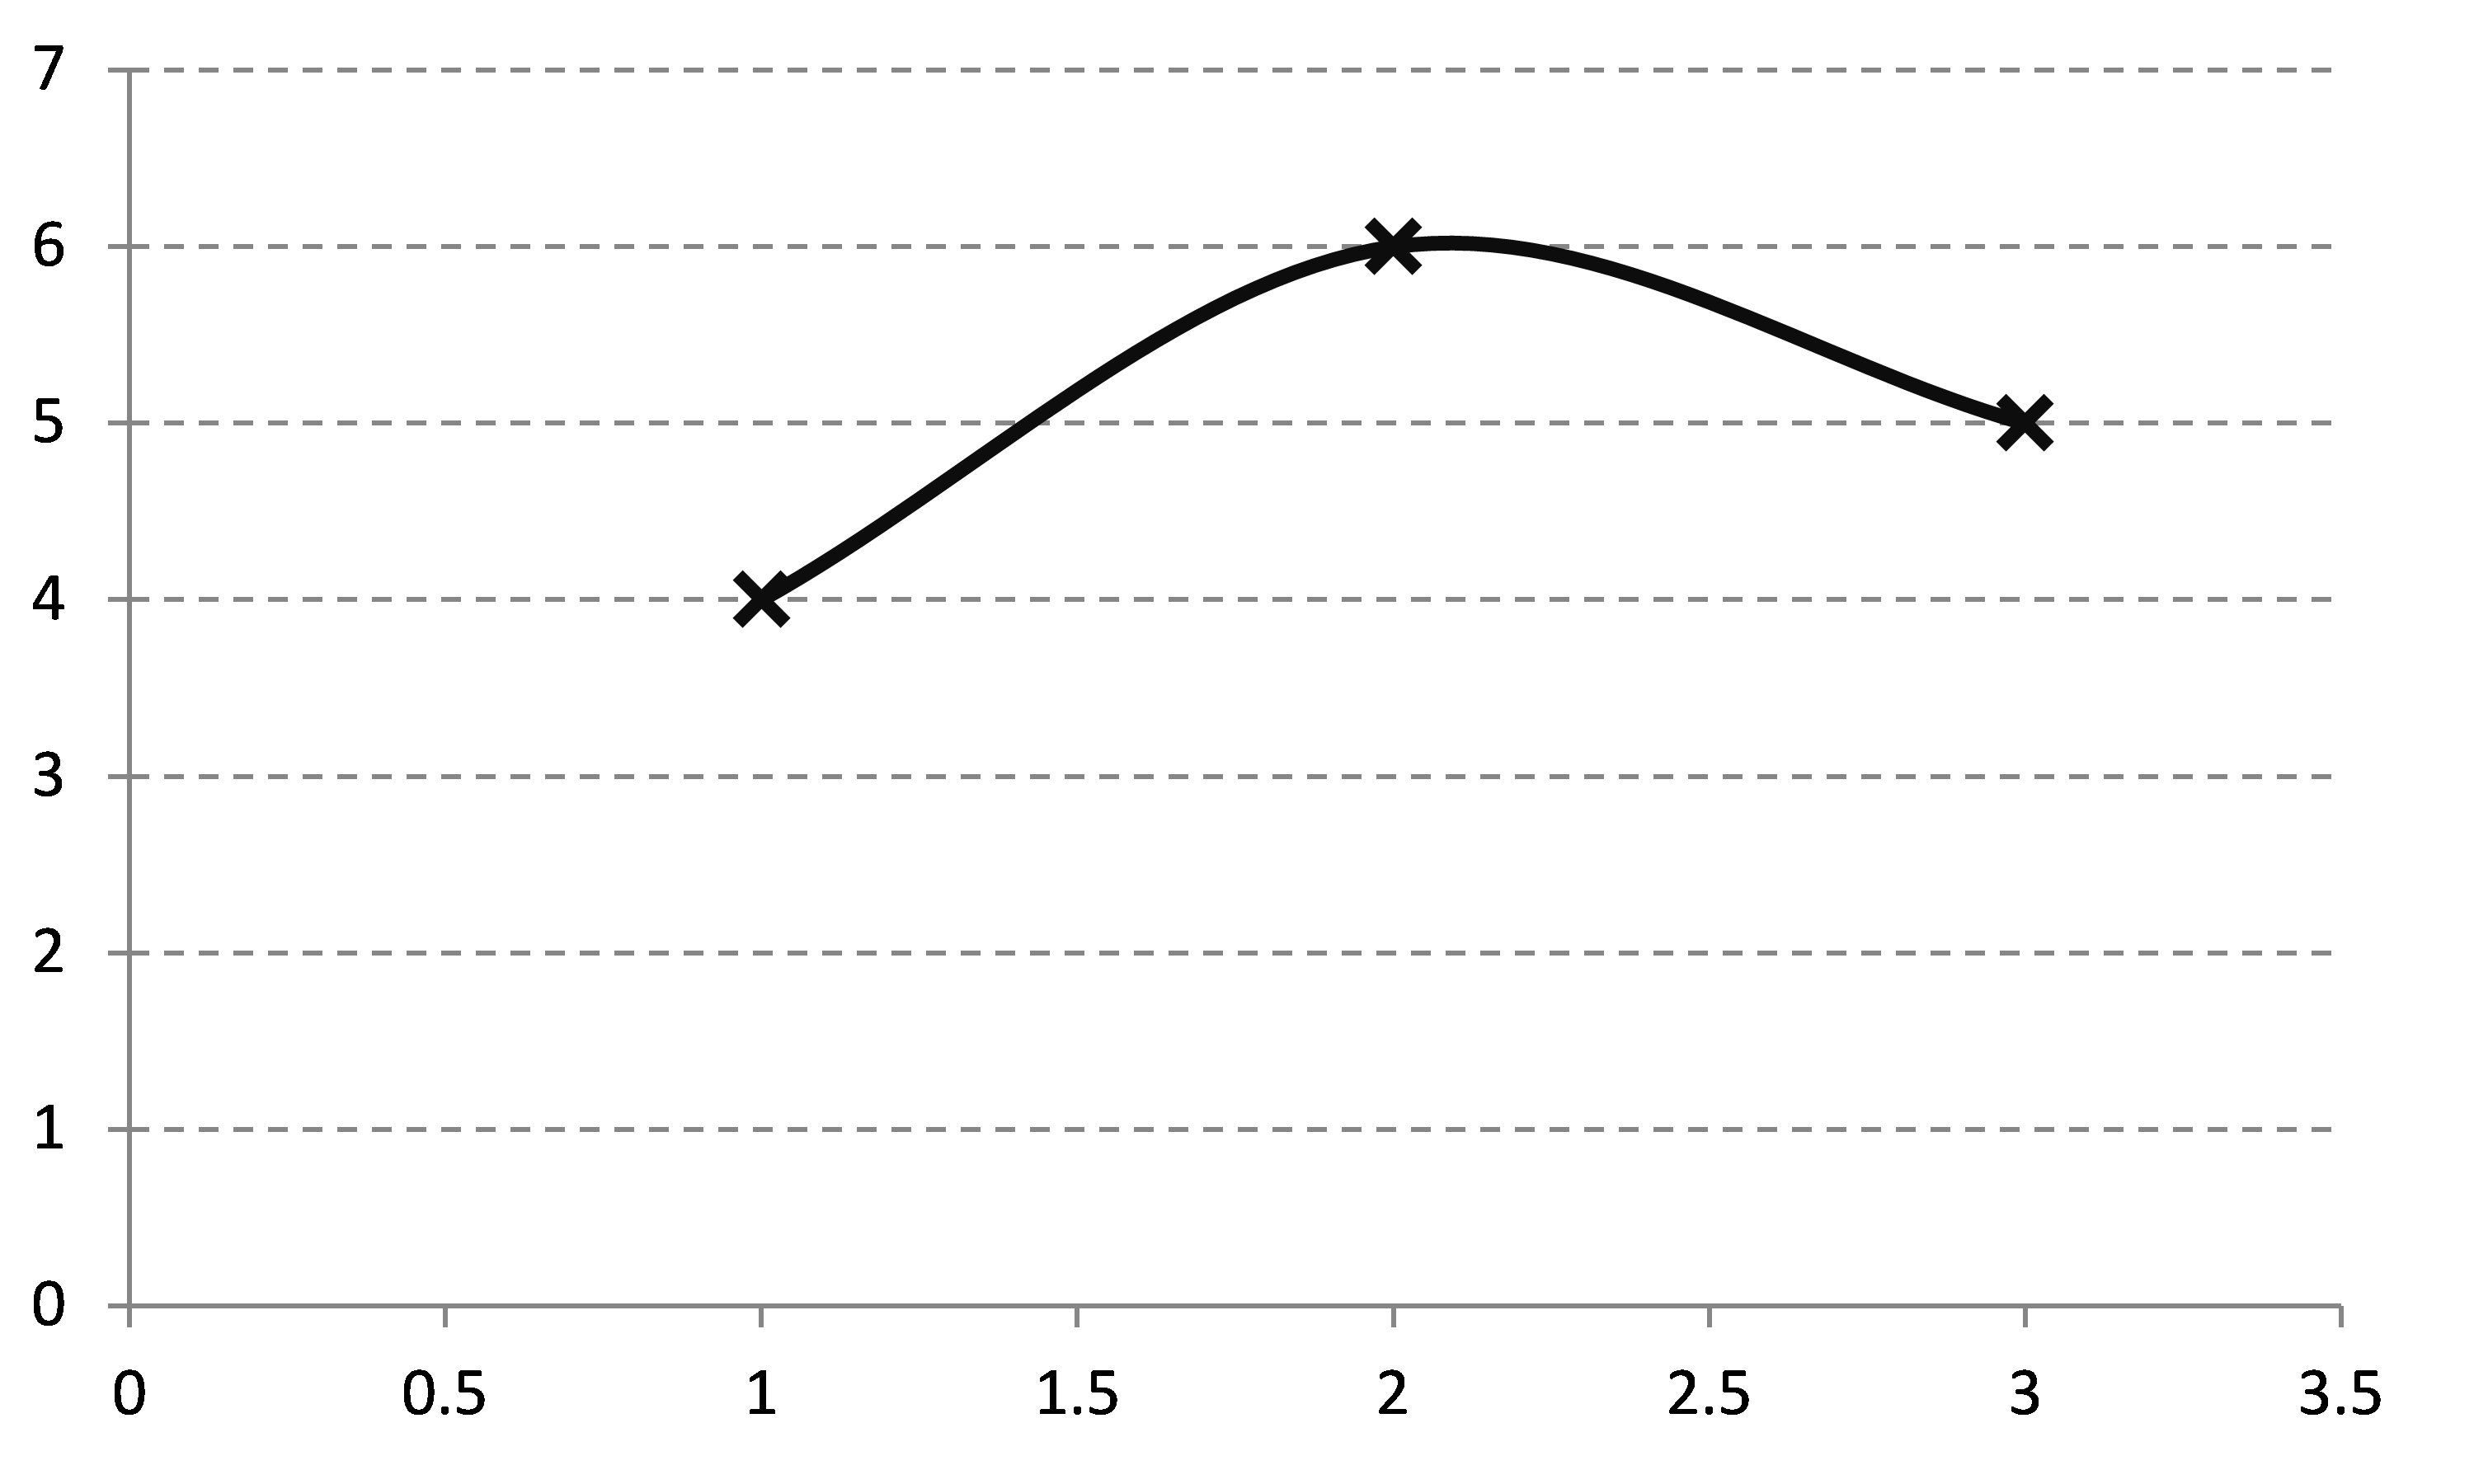
\includegraphics[width=0.6\textwidth]{beautifulgraph.png}
		\caption{\colorbox{green}{Figure caption – below the figure}}
		\label{fig:dumber}
\end{center}
\end{figure}

\colorbox{yellow}{Text.}\par
\subsection{\colorbox{green}{Subtitle if needed}}
\colorbox{green}{Subsection text}
\subsection{\colorbox{green}{Subtitle if needed}}
\colorbox{green}{Subsection text}


\section{Conclusions}
\addcontentsline{toc}{section}{Conclusions}
\colorbox{yellow}{Text.}\par

% \cite*{} actually, that's a dirty trick here... but just for generating the AUX file
% (references in the preamble are not recognised)

\bibliographystyle{unsrtnat}
\renewcommand{\refname}{References}
\addcontentsline{toc}{section}{References}

\def\bibpreamble{{\color{red}Please provide the references in order of appearance in the text. Refer to them in the text by means of the sequential numbers in brackets generated below, {\it e.g.} using the allowed citation style.
Using the provided package, you can for instance refer to the work of~\citet{Lamport89}, without forgetting to mention the Code of Practice~\cite{CodePractice18} as well as the essential work of~\citet{Rumsey15}. Altogether, we shall further expand the work of~\cite{Cohen38}.}
}% no need for preamble

%%\printbibliography % when using biblatex

\bibliography{\thisfile.bib}

\end{document}